% T35 — «Японский ваби-саби»: асимметричная вёрстка, серый акцент, дыхание полей.
% Math, класс 10, 5 задач с большим левым/правым полем «дыхания».
\documentclass[a4paper,11pt]{article}

\usepackage{../../../../Lessons/_templates/preamble_worksheet}
\usepackage{../_shared/worksheet_check}

% Геометрия: широкое правое поле — асимметрия в духе ваби-саби.
\geometry{a4paper, top=22mm, bottom=22mm, left=22mm, right=58mm}

% --- Палитра: приглушённый сумиэ-серый + тонкий чернильный мазок ---
\definecolor{wcprimary}{HTML}{4A4A4A}
\definecolor{wcprimaryLight}{HTML}{D9D6D2}
\definecolor{wcprimaryBG}{HTML}{FAF8F4}
\definecolor{wcsumi}{HTML}{2B2B2B}
\definecolor{wcaccent}{HTML}{8E7B5C}

\renewcommand{\familydefault}{\sfdefault}

% --- Заголовок: одинокий иероглифический штрих и тонкий текст ---
\renewcommand{\WorksheetTitle}[1]{%
  \par\noindent\begin{tikzpicture}
    % Один мазок-«штрих» слева сверху, наклонный, неровный
    \draw[wcsumi, line width=2.2pt, line cap=round]
      (0,0) .. controls (4mm,-1mm) and (8mm,-2mm) .. (14mm,-3mm);
    \draw[wcsumi, line width=1.2pt, line cap=round]
      (1mm,-2mm) -- (5mm,-2.5mm);
    % Заголовок: лёгкий, без рамки
    \node[anchor=west, text=wcsumi, font=\fontsize{16pt}{18pt}\selectfont]
      at (20mm, -2mm) {#1};
  \end{tikzpicture}\par\vspace{2mm}
  % Тонкая горизонтальная линия, не доходящая до правого края
  \noindent\textcolor{wcprimaryLight}{\rule{0.55\linewidth}{0.4pt}}\par\vspace{6mm}}

% Асимметричная задача: висячий отступ слева, ответ глубоко справа.
\newcommand{\WabiTask}[2]{% #1 номер #2 содержимое
  \par\vspace{3mm}
  \begingroup
  \leftskip=10mm
  \hangindent=12mm
  \hangafter=1
  \noindent
  {\fontsize{9pt}{10pt}\selectfont\color{wcaccent}\textbf{\textsf{#1}}}\quad
  {\color{wcsumi}#2}\par
  \endgroup}

\SetAnswerFieldSize{30mm}{7mm}

% --- FirstPageHeader: тонкий, минималистичный ---
\renewcommand{\FirstPageHeader}{%
  \par\noindent
  {\footnotesize\color{wcprimary}
    \textsf{Имя}\;\textcolor{wcprimaryLight}{\rule{45mm}{0.3pt}}\hfill
    \textsf{Класс}\;\textcolor{wcprimaryLight}{\rule{12mm}{0.3pt}}\hfill
    \textsf{Дата}\;\textcolor{wcprimaryLight}{\rule{22mm}{0.3pt}}}\par
  \vspace{6mm}}

\begin{document}

\WorksheetTitle{Тишина чисел}
\par\noindent{\footnotesize\color{wcprimary!85}\textsf{Класс 10 \quad·\quad T35 \quad·\quad ID: T35-wabi-2026-05-27}}\par\vspace{2mm}
\FirstPageHeader

\WabiTask{01}{%
  Найдите наименьшее значение функции $y = x^3 - 6x^2 + 9x + 1$ на отрезке $[0;\,5]$.\par
  \vspace{1.5mm}\hspace*{12mm}\textsf{\footnotesize\color{wcaccent}ответ}\;\;\AnswerField{1}%
}

\WabiTask{02}{%
  Решите уравнение $\log_3(x^2 - 2x) = 1$. В ответе укажите больший корень.\par
  \vspace{1.5mm}\hspace*{12mm}\textsf{\footnotesize\color{wcaccent}ответ}\;\;\AnswerField{2}%
}

\WabiTask{03}{%
  Вычислите $\dfrac{\sin 75^\circ - \sin 15^\circ}{\cos 75^\circ + \cos 15^\circ}$.\par
  \vspace{1.5mm}\hspace*{12mm}\textsf{\footnotesize\color{wcaccent}ответ}\;\;\AnswerField{3}%
}

\WabiTask{04}{%
  В правильной треугольной призме сторона основания равна $4$, а боковое ребро равно $3$.
  Найдите объём призмы.\par
  \vspace{1.5mm}\hspace*{12mm}\textsf{\footnotesize\color{wcaccent}ответ}\;\;\AnswerField{4}%
}

\WabiTask{05}{%
  Геометрическая прогрессия задана условиями $b_1 = 2$, $q = 3$.
  Найдите сумму первых пяти членов прогрессии.\par
  \vspace{1.5mm}\hspace*{12mm}\textsf{\footnotesize\color{wcaccent}ответ}\;\;\AnswerField{5}%
}

\vspace{8mm}
% Финальный «штрих»: одинокий мазок справа внизу — пустота как акцент.
\noindent\hfill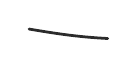
\begin{tikzpicture}
  \draw[wcsumi, line width=1pt, line cap=round]
    (0,0) .. controls (3mm,-0.5mm) and (6mm,-1mm) .. (10mm,-1.2mm);
\end{tikzpicture}

\WorksheetQR{T35-wabi/L1/v1}

\end{document}
